\documentclass[16pts]{report}
\usepackage[utf8]{inputenc}
\usepackage[T1]{fontenc}
\usepackage[francais]{babel}
\usepackage{xcolor}
\usepackage[hyphens]{url}
\usepackage[hidelinks]{hyperref}
\usepackage{amsmath}
\usepackage{graphicx}
\usepackage{geometry}
\usepackage{textcomp}
\hypersetup{hypertexnames=true}
\geometry{hmargin=2.5cm,vmargin=1.5cm}

\usepackage{float} %Option H pour les figures, utile.

%\maketitle
%\clearpage

\begin{document}
\bibliographystyle{unsrt}
\nocite{*}

\chapter{Evolutions}
\label{cha:Evolutions}

\section{Evolution des besoins}
\label{sec:Evolution des besoins}

Durant la phase de conception de notre projet, nous nous sommes confronté à 
deux difficultés qui ont fait évoler nos besoins. En effet, nos recherches 
nous pas permis de pouvoir résoudre les conflits automatiquement ni de générer 
une configuration par défaut en fonction du matériel de l'utilisateur, comme
cela a été évoqué précédemment. 
\\
L'objectif de résolution automatique des conflits a été modifié afin de 
simplement aider l'utilisateur à trouver les conflits d'une option. Il se 
chargera de modifier les valeurs des options par lui-même.
\\
En ce qui concerne le besoin de détecter la matériel d'un utilisateur, celui-ci 
s'est transformé pour devenir une base de donnée communautaire. Celle-ci est 
modifiable à l'aide d'un site web. Il est possible d'ajouter des relations 
entre des options et des modules, et entre des modules et du matériels. Les 
modules représentent la partie Driver. Un second besoin était de pouvoir 
ajouter des Tags aux options afin de pouvoir les regrouper afin d'affiner la 
recherche. Ce besoin a également été ajouté sur cette base communautaire.

AJOUTER une photos du SITE

AJOUTER un petit diagramme des classes

(On verra quand le site aura avancé)

\section{Evolution de l'interface}
\label{sec:Evolution de l'interface}

En parallèle de l'évolution des besoins, l'ergonomie de l'interface a changé 
afin d'améliorer l'utilisation de l'application et afin de correspondre aux 
fonctionnalités attendues.

\begin{enumerate}

	\item Evolution de l'interface de configuration de l'application
	\\

	L'interface de configuration permet à l'utilisateur de choisir le noyau 
	et l'architecture qu'il désire. Il peut également charger un fichier de 
	configuration existant.

	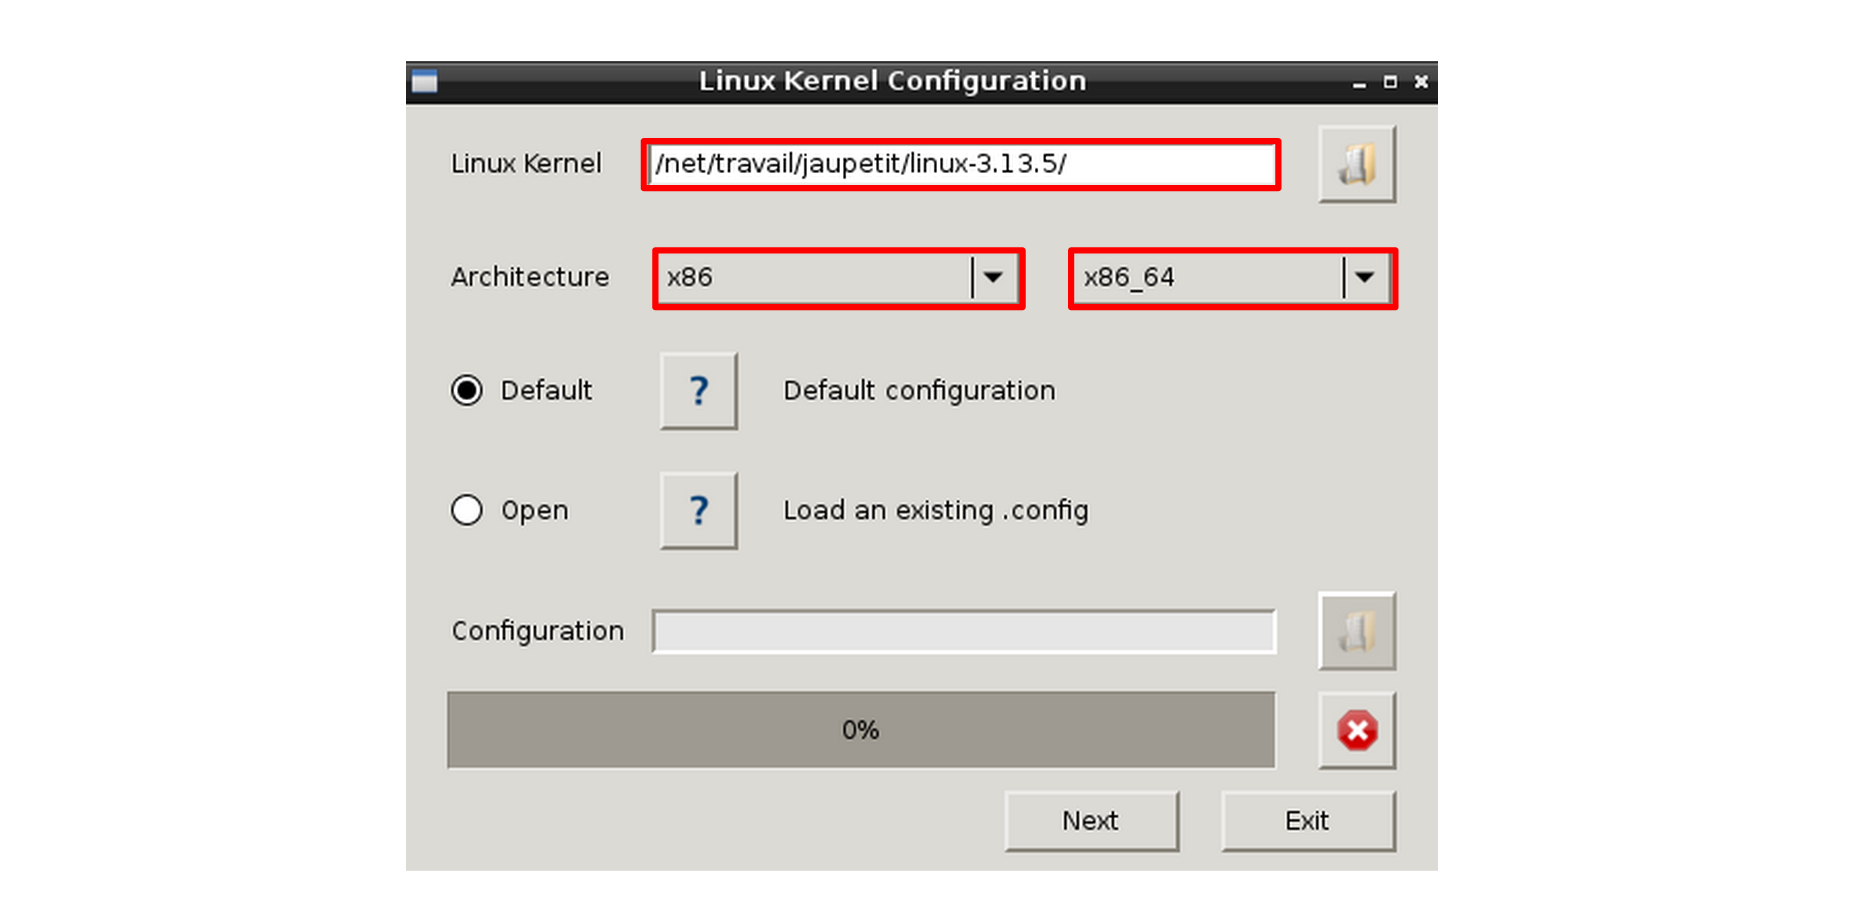
\includegraphics[scale=0.5]{illustrations/screen_configuration_interface.png}
	\centering
	\caption{Evolution de l'interface de configuration de l'application}
	\label{fig:Evo_config}

	L'utilisateur n'a plus que deux choix contre quatre auparavant. En effet, 
	il ne peut plus détecter son matériel automatiquement comme cela était 
	le cas sur les maquettes. Il ne peut plus créer une configuration vierge 
	car certaines options sont nécessaire pour ne pas créer de conflits.


	L'interface modification des options autorise l'utilisateur à naviguer 
	entre les options avec différents menus. Il peut modifier leurs valeurs 
	s'il n'y a pas de conflit et générer un fichier de configuration lors 
	qu'il a terminé.

	\item Evolution de l'interface d'affichage des options
	\\
	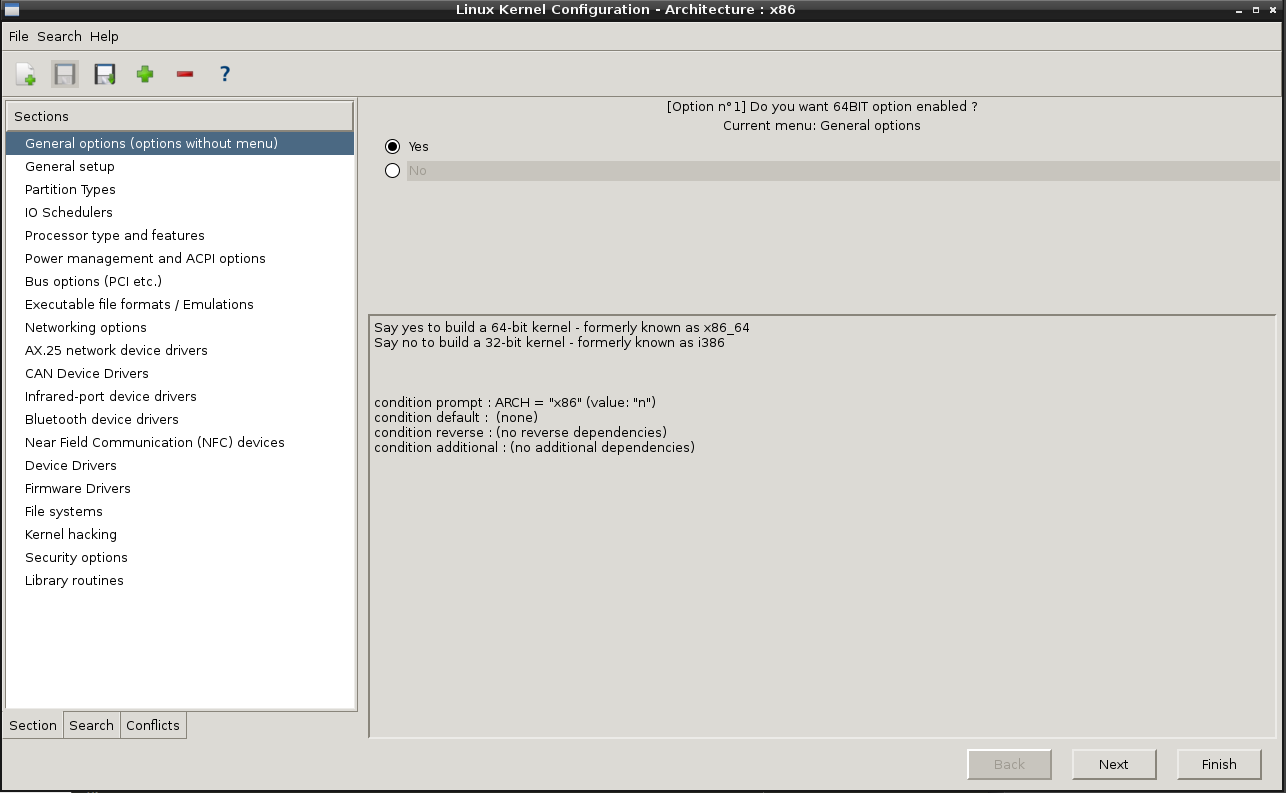
\includegraphics[scale=0.5]{illustrations/screen_options_interface.png}
	\centering
	\caption{Evolution de l'interface d'affichage des options}
	\label{fig:Evo_config}



	\item Evolution de l'interface de recherche des options
	\\
	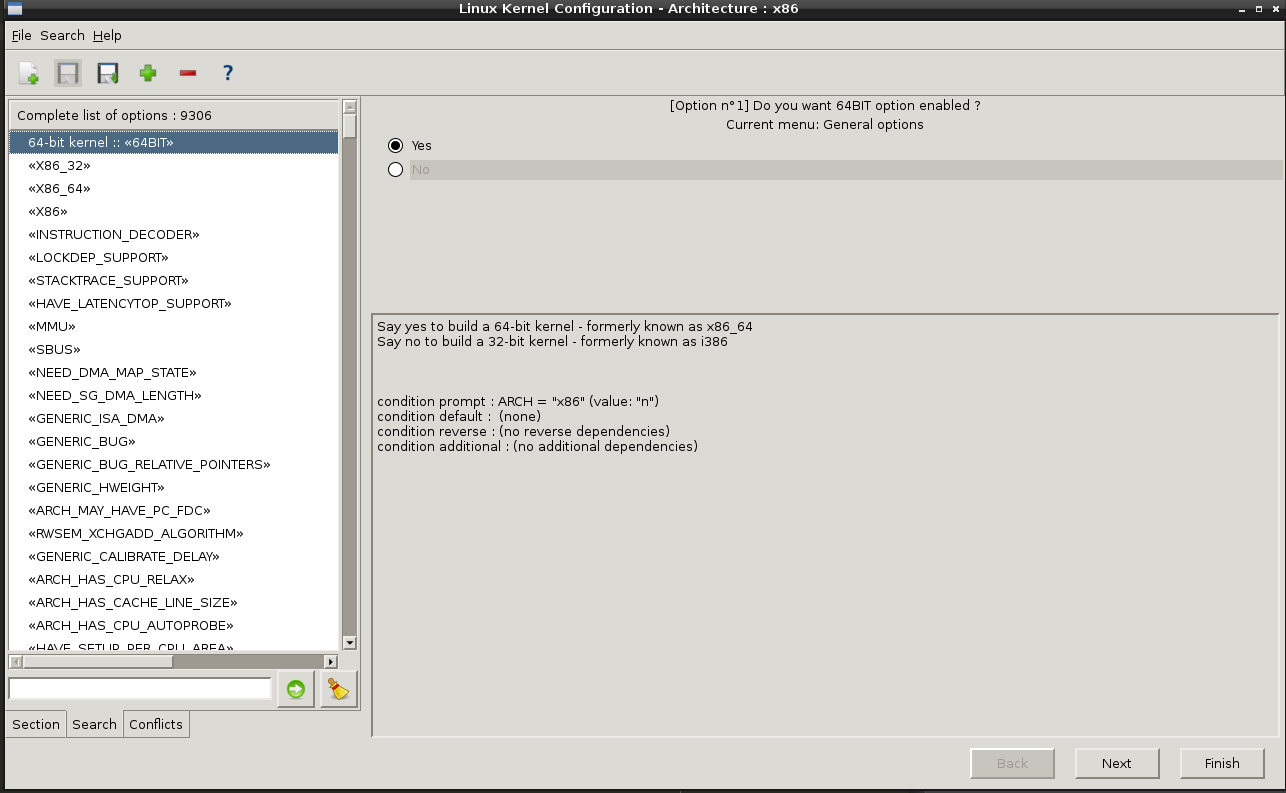
\includegraphics[scale=0.5]{illustrations/screen_options_search_interface.png}
	\centering
	\caption{Evolution de l'interface de recherche des options}
	\label{fig:Evo_config}



	\item Evolution de l'interface d'affichage des conflits
	\\
	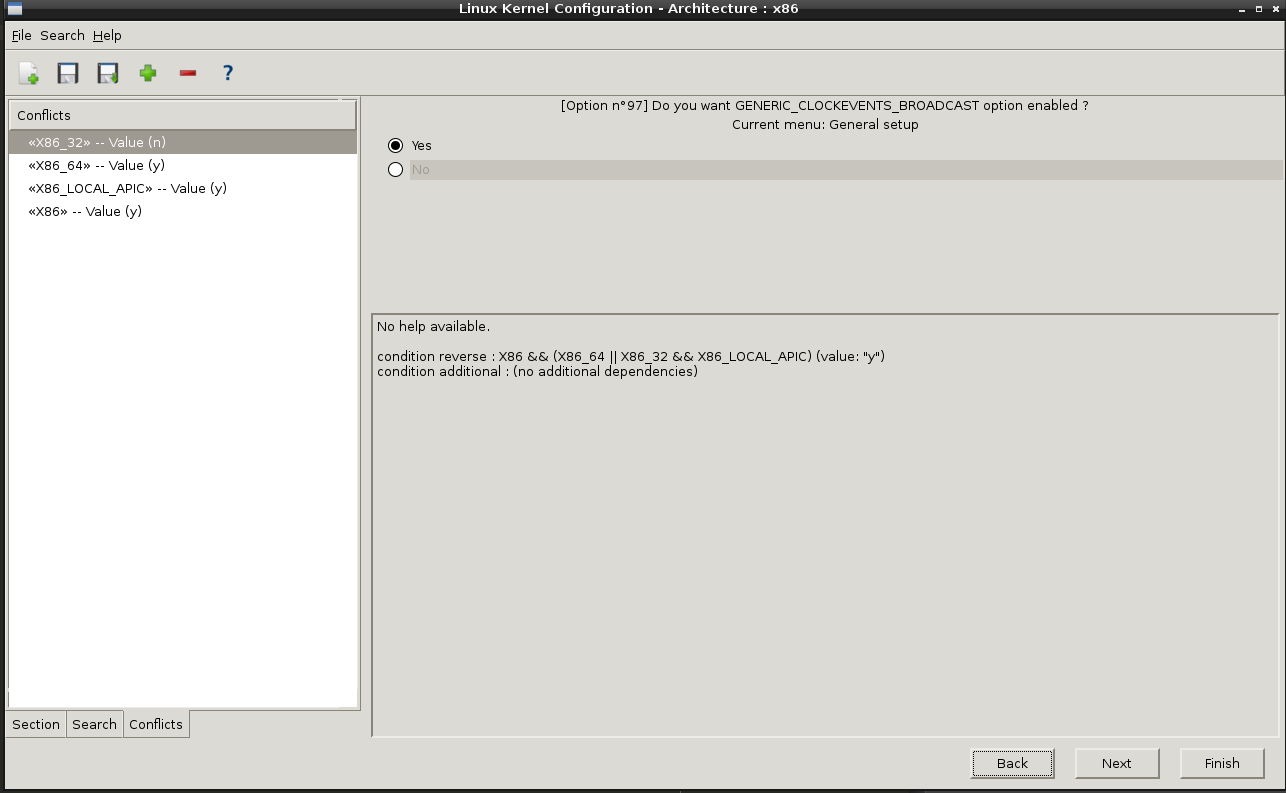
\includegraphics[scale=0.5]{illustrations/screen_options_conflits_interface.png}
	\centering
	\caption{Evolution de l'interface d'affichage des conflits}
	\label{fig:Evo_config}


\end{enumerate}

\end{document}
